\chapter{Bootstrapped Active Curricula}\label{ch:BootstrappedActiveCurricula}
The first curriculum construction approach we investigate is what we term \textit{bootstrapped active curricula (BAC)}, the name is chosen as it involves `bootstrapping' a curriculum from a separate model. The intuition behind this approach is that, while it may be difficult to ascertain a-priori which samples are `hard' or `easy' (particularly for very large datasets where it is infeasible to analyse every sample), we can automatically infer which samples are difficult by first training a model on the data and then using an active learning uncertainty metric to investigate which samples the model is uncertain about classifying. Using prediction uncertainty to approximate difficulty, we can then construct a learning curriculum which can be used to train a new model, for example by splitting the training samples into separate tasks of increasing difficulty, as detailed below.
\section{Curriculum Construction}
In the BAC approach we train two models; the first, which we term the `baseline model' and denote  $\theta_{baseline}$, is trained to convergence using a standard mini-batch gradient descent optimisation on the entire available training set $\mathcal{T}$. We then use $\theta_{baseline}$ in conjunction with the Absolute Average Distance to Threshold uncertainty function as defined below in Section \ref{BAC_AADT}, scoring each training sample in $\mathcal{T}$. This produces $\mathbf{S}^{\theta_{baseline}}$, a vector of $N$ scores, where $N$ is the number of samples in $\mathcal{T}$, such that the $i^{th}$ element of $\mathbf{S}^{\theta_{baseline}}$ is the output of the AADT uncertainty function for the $i^{th}$ training sample inputs:

\begin{equation}\label{eq:BAC_S}
S^{\theta_{baseline}}_i = AADT_{\theta_{baseline}}(x_i) 
\end{equation}
where $x_i$ are the inputs of the $i^{th}$ training sample. We then abuse the function notation slightly to set $\mathbf{S}^{\theta_{baseline}} = AADT_{\theta_{baseline}}(\mathcal{T}) $, i.e. signifying that $\mathbf{S}^{\theta_{baseline}} $ is the output of the AADT uncertainty function over the entire training set $\mathcal{T}$.

 We then sort the training samples according to their score, producing an ordered training set $\mathcal{T}_{\mathbf{S}^{\theta_{baseline}}}$, such that the first training sample in $\mathcal{T}_{\mathbf{S}^{\theta_{baseline}}}$ is the sample which produces the highest value from the AADT function. We then split $\mathcal{T}_{\mathbf{S}^{\theta_{baseline}}}$ into equally sized `tasks', with the number of tasks being a hyperparameter of the curriculum construction. The learning curriculum is then constructed from these tasks; the chosen approach is to split training into discrete phases, with the number of phases being equal to the chosen number of tasks. The first phase of the curriculum consists of training only on the first task, denoted $\mathcal{T}^1_{\mathbf{S}^{\theta_{baseline}}}$, in the second phase, the second task is added to the training samples, training the model on $\mathcal{T}^1_{\mathbf{S}^{\theta_{baseline}}}\cup\mathcal{T}^2_{\mathbf{S}^{\theta_{baseline}}}$. In the third phase (if the number of tasks is greater than 2), the next task is added, and so on until all tasks have been added and the final phase consist of training on the entirety of the original training set $\mathcal{T}$. Having constructed the BAC learning curriculum, we train a new `curriculum' model', which we denote by $\theta_{curriculum}$, using the curriculum. Pseudocode for the BAC method is given in Section \ref{BACPseudocode}.

\subsection{Average Absolute Distance to Threshold (AADT)}\label{BAC_AADT}
A popular active learning uncertainty method is to examine the proximity of the model's outputs to the classification bounday. The assumption is that samples that the model is uncertain about classifying will produce probabilities close to the classification boundary; indeed as mentioned in Section \ref{Background_ActiveLearning} the authors of \cite{Chang18} show that prediction variance is inversely proportional to the distance to the boundary. From a curriculum perspective we can estimate a sample's difficulty by the algorithm's uncertainty in predicting the class label, with uncertain samples being seen as hard, and vice versa. We thus define the uncertainty function $AADT$ which calculates the absolute distance to classification threshold for the model outputs, averaged across all possible classes. Note that the function is dependent on a the output of the model in question, which is denoted $\theta$.
\begin{equation}
AADT_{\theta}(x_i) = \frac{ \sum_{c=1}^{C} \left|P_{\theta}(y_c |x_i) - \frac{1}{C}\right|}{C}.
\end{equation}
Where $|.|$ represents the L1 norm/absolute value function.
Here $N$ is the number of training samples, $C$ is the number of output classes and $P_{\theta}(y_c |x_i)$ is the output softmax probability for class $y_c$ of the model $\theta$, given input $x_i$. We also tested the average \textit{square} of the distance to threshold, as opposed to the absolute distance to threshold, as well as testing the entropy of the outputs as an uncertainty measure, however results were extremely similar in all cases.

\subsection{Phase Training Epochs}
A naive approach to the BAC approach would be to train the curriculum model for the same number of epochs as the baseline model, split equally acrossing training phases. For example if the baseline model was trained for 100 epochs and we then constructed a two task curriculum, the curriculum model would be trained on the first task for the first 50 epochs, then on both tasks for the second 50 epochs. The issue with this method however is that, as during the first 50 epochs there are only half as many training samples, the curriculum model will not have as many parameter updates as the baseline model. To emphasize this, consider that if we were using stochastic gradient descent (i.e. a mini-batch size of 1) with a full training set of 1000 samples, the baseline model in this instance would have (\# epochs * \# training samples) parameter updates, i.e. 100 * 1000 = 100,000 parameter updates. The curriculum model on the other hand would have (50*500) parameter updates the first training phase and (50*1000) in the second, resulting in a total of   (50*500) + (50*1000) = 75,000 parameter updates, 25\% less updates than the baseline model. To address this, we increase the number of epochs in each phase by the ratio of the number of samples used in the phase to the size of the whole training set. Specifically, we set the number of training epochs in each phase as follows:
\begin{equation}\label{eq:BAC_Epochs}
NumEpochs^{t} =\floor{ \frac{BaselineEpochs}{t}}
\end{equation}
Where $BaselineEpochs$ is the number of epochs used to train the baseline model and $NumEpochs^{t}$ denotes the number of training epochs in the $t^{th}$ training phase. For example, in the first phase, $NumEpochs^{1} = \frac{BaselineEpochs}{1} = BaselineEpochs$. $\floor{.}$ represents the floor function; as $\frac{BaselineEpochs}{i}$ will not always be integer, we round down the number of epochs in each phase. The curriculum model will therefore be trained for a higher number of epochs (precisely, $\sum_{t=1}^{NumTasks}{\frac{1}{t}}$ times more epochs), however the number of parameter updates will be equalised. 

\subsection{Pseudocode for BAC}\label{BACPseudocode}
Pseudocode for the boostrapped active curriculum method (assuming the use of the AADT uncertainty function and an easy to hard curriculum):
\begin{algorithmic}
\FOR {$Num\_Epochs$}
\STATE $\text{train }  \theta_{baseline} \text{ on training set } \mathcal{T}$
\ENDFOR
\STATE $\mathbf{S}^{\theta_{baseline}} = AADT_{\theta_{baseline}}(\mathcal{T})$
\STATE $\mathcal{T}_{\mathbf{S}^{\theta_{baseline}}} = \mathcal{T}, \text{sorted by } \mathbf{S}^{\theta_{baseline}} \text{ (descending order)}$ 
\STATE $Num\_Samples = |\mathcal{T}_{\mathbf{S}^{\theta_{baseline}}}|$
\FOR {$t=0$ to $Num\_Tasks$}
\STATE $TaskStartIndex = Num\_Samples*\frac{t}{Num\_Tasks} $
\STATE $TaskEndIndex = Num\_Samples*\frac{t+1}{Num\_Tasks} $
\STATE $\mathcal{T}^{t}_{\mathbf{S}^{\theta_{baseline}}} = \mathcal{T}_{\mathbf{S}^{\theta_{baseline}}}[TaskStartIndex:TaskEndIndex,:] $
\ENDFOR
\FOR {$t=0$ to $Num\_Tasks$}
\STATE $Num\_Epochs\_Task = \floor{\frac{Num\_Epochs}{t}}$
\FOR{$Num\_Epochs\_Task$}
\STATE $\text{train }  \theta_{curriculum} \text{ on training set } \mathcal{T}^{0:t}_{\mathbf{S}^{\theta_{baseline}}} $
\ENDFOR
\ENDFOR
\end{algorithmic}

\section{Geometric Shapes Dataset}\label{sec:GeoShapes}
To test the boostrapped active curriculum approach we use the `Geometric Shapes' dataset \cite{GeoShapes}, as used in \cite{Bengio2009}. This dataset consists of 32x32 pixel images of geometric shapes, specifically ellipses, rectangles and triangles; the class labels are one-hot vectors which indicate to which of the three classes each sample belongs. As well as varying the shapes shown in the image, the samples also vary in colour, orientation, size and position. This dataset is used in \cite{Bengio2009} as it is easy to construct a predefined curriculum for geometric shapes; circles, squares and equilateral triangles represent regular, `easy' versions of the broader classes of ellipses, rectangles and triangles, respectively. The authors of \cite{Bengio2009} train a curriculum model by first training only on an easy training set consisting only of circles, squares and equilateral triangles, before then training on a hard training set with the more general shapes. The easy and difficult training sets consist of 10,000 training samples, giving a total of 20,000 training samples, while the test set, consisting only of hard samples, contains 5,000 images. The authors demonstrate that their approach outperforms an identical model trained only on the harder shapes; the curriculum model consistently achieves greater test accuracy, with the greatest improvement coming  when the first half of the training epochs train on the easier shapes, and the second half the harder ones, as shown in Figure 3 of their paper. As discussed by the authors, one potential pitfall of their experiments is that the curriculum model has seen more samples than the benchmark model, as it has been trained on both the easy and the difficult training sets, to avoid this in our experiments, the training set we use is the union of both the easy and difficult samples. Our training set therefore consists of 20,000 geometric shape images, including both the easy, regular shapes and the more difficult shapes, the test set is unchanged however, consisting of the 5,000 difficult samples. 

Some example images for the Geometric Shapes dataset are given in Figure \ref{fig:GeoSamples} below, with Figure \ref{fig:EasyGeoSamples} showing examples from the easy training set featuring circles, squares and equilateral triangles, while Figure \ref{fig:HardGeoSamples} shows samples from the more difficult training set of general shapes.

\begin{figure}
\hspace*{-2cm}    
\centering
\begin{subfigure}{.6\textwidth}
  \centering
  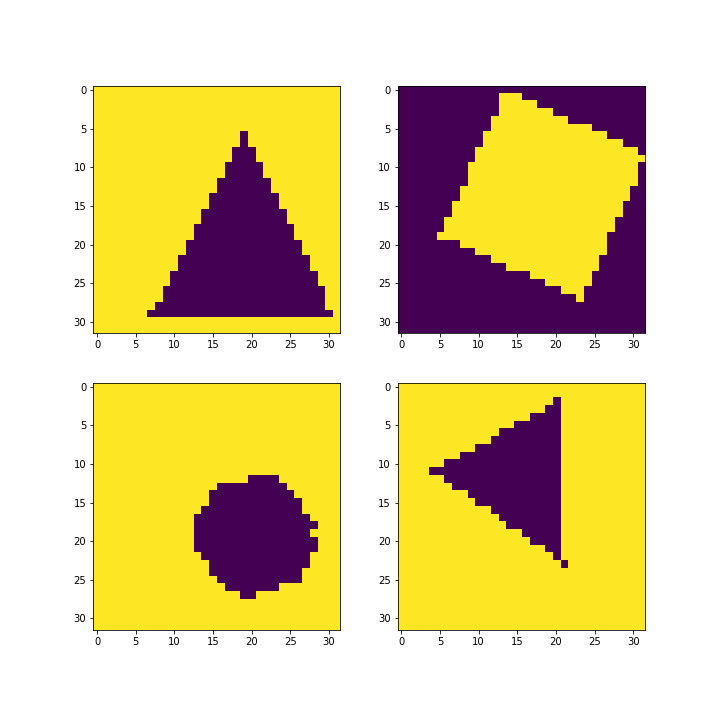
\includegraphics[width=1\linewidth]{EasyGeoShapesExamples.png}
  \caption{Samples from `easy' training set}
  \label{fig:EasyGeoSamples}
\end{subfigure}%
\begin{subfigure}{.6\textwidth}
  \centering
  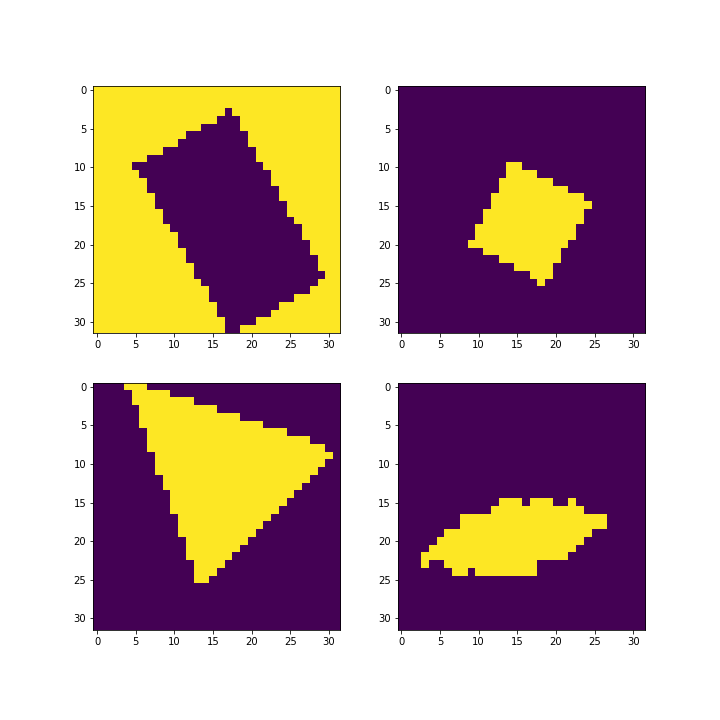
\includegraphics[width=1\linewidth]{HardGeoShapesExamples.png}
  \caption{Samples from `hard' training set}
  \label{fig:HardGeoSamples}
\end{subfigure}
\caption{Sample figures from the Geometric Shapes dataset}
\label{fig:GeoSamples}
\end{figure}

 In the results Section \ref{sec:BAC_Results}, we analyse how succesful our tested curriculum method is at automatically identifying which samples come from the easy or hard training sets, investigating which training samples fall into the different tasks automatically constructed through the BAC curriculum method. 

\section{Experiments}
 In order to measure the effect of the curriculum on test performance, we set $\theta_{baseline}$ and $\theta_{curriculum}$ to have identical architectures, hyperparameters and initial weights, essentially minimizing any differences in training besides the learning curriculum. We use both the Average Absolute Distance to Threshold (AADT) function, detailed in Section \ref{BAC_AADT}, to score the training samples with the trained baseline model in each experiment. Furthermore, as well as testing `easy to hard' curricula, where the training phases progress from  $\mathcal{T}^1_{\mathbf{S}^{\theta_{baseline}}}$ to the final task, we also test the opposite approach, with the first training phase using only the hardest task, then incorporating the other, easier tasks throughout training. We run the experiments using the Geometric Shapes dataset, as introduced in Section \ref{sec:GeoShapes}, allowing us to compare results with the predefined curriculum as in \cite{Bengio2009}. To do so, as well as training the baseline and BAC curriculum models, we also train a model using the predefined curriculum method laid out in \cite{Bengio2009}, specifically training on only the easy samples in for the first half of the training epochs, and only the hard samples in the second half. In order to better compare the predefined curriculum method from \cite{Bengio2009}, we also run an adjusted version of their method; unlike the BAC approach, where we correct the difference in number of parameter updates between the curriculum model and the baseline model, the predefined curriculum model will end up undergoing significantly less parameter updates than our baseline (in fact it will have half as many updates). We therefore correct for this in two ways; in the first phase of training, in which the model is trained only on the easy images, lasts for twice as many epochs as in the unadjusted method (correcting for the fact that it consists of half as many samples as the full training set). The second phase of the adjusted model is then trained on the \textit{full} training set, consisting of the union of the hard and easy samples. This should allow for a better comparison between the BAC models, the baseline model, and the predefined curriculum approach. We therefore train 5 separate models:
 \begin{itemize}
 \item Baseline Model - Trained on the full training set of easy and hard geometric shape images for all epochs, with standard mini-batch stochastic gradient descent.
 \item Easy to Hard Model - Trained with a boostrapped active curriculum construct from the above Baseline Model, beginning with the easiest/least uncertain task and including the other tasks throughout training.
 \item Hard to Easy Model - As above, but training begins with the hardest/most uncertain tasks before incoporating the easier tasks throughout training.
 \item Predefined Curriculum - As in \cite{Bengio2009}, the first half of the training epochs use only the 10,000 easy training samples, while the second half train on only the 10,000 hard training samples.
 \item Adjusted Predefined Curriculum - As above, but the number of epochs in the first phase of training is doubled to account for the difference in parameter updates, and the second phase uses both easy and hard training samples for better comparison with the BAC models.
 \end{itemize}
 
All models are tested on the same test set of 5000 images, all containing `hard' geometric shapes; experiments are repeated multiple times with different weight initialisations. To analyse the effect of the curriculum on learning we report the accuracy and cross-entropy error of the different models over the held out test set. The exact model architecture is given in tables 5.1 - 5.3 below (`FC' = fully connected Layer):
 
\begin{table}[h]
\caption{Geometric Shapes Dataset Model Architecture} \label{tab:GeoArchitecture}
\begin{tabular}{|c||c|c|c|c|c|c|c|}
\hline
\multicolumn{8}{|c|}{Geometric Shapes Dataset Model Architecture} \\
\hline
 & Layer 1 & Layer 2 & Layer 3& Layer 4 &Layer 5 & Layer 6 & Layer 7 \\
\hline
Layer Type & FC & Dropout & FC & Dropout & FC & Dropout  & FC \\
\hline
Units & 300 & NA & 300 & NA & 300 & NA & 3 \\
\hline
Activation & Tanh \footnotemark & NA & Tanh & NA & Tanh & NA & Softmax \\
\hline
\end{tabular}
\end{table}
\footnotetext{The Hyperbolic Tangent activation is chosen as this was this the activation used in \cite{Bengio2009}.}
We also lay out the hyperparameters for the training procedures in table \ref{tab:HyperParams} below, experiments were carried out in Keras \cite{chollet2015keras} with the Adam optimiser implemented with the default hyperparameters (except for the learning rate which is given in Table \ref{tab:HyperParams}):

\begin{table}[h]
\caption{Experiment Hyperparameters} \label{tab:HyperParams}
\begin{tabular}{|c||c|c|c|c|c|c|}
\hline
\multicolumn{7}{|c|}{Experiment Hyperparameters} \\
\hline
 &Epochs & Optimiser &Learning Rate & Dropout \% & Batch Size & Num Tasks \\
\hline
GeoShapes & 350 & Adam & 0.0001 & 0.25 & 32 & 2  \\
\hline
\end{tabular}
\end{table}


Architectures and hyperparameters were chosen and tuned in order to deliver a good level of performance without prohibitive training times, robustness tests were however carried out varying the model architectures and hyperparameters resulting in little change in the relative performance of the different methods. 
\section{Results and Discussion}\label{sec:BAC_Results}
The results of running the bootstrapped active curriuculum experiments with the Geometric Shapes dataset are summarised in Table \ref{tab:GeoShapes BACResults} and Figure \ref{fig:GeoShapesBACResults} which shows the test set accuracies and cross entropy errors, including standard errors, derived from 24 experiments with different initialisations.
\begin{table}[h]
\caption{Geometric Shapes BAC Results} \label{tab:GeoShapes BACResults}
\begin{tabular}{|c||c|c|}
\hline
\multicolumn{3}{|c|}{GeoShapes BAC Results} \\
\hline
 & Test Accuracy (\%) & Test Cross-Entropy Error \\
\hline
Uniform Baseline&  0.825 $\pm$ 0.00269 & 0.440 $\pm$ 0.00614 \\
\hline
Easy to Hard Curriculum & 0.840 $\pm$ 0.00267 & 0.398 $\pm$ 0.00670 \\
\hline
Hard to Easy Curriculum &  0.815 $\pm$ 0.00278 & 0.467 $\pm$ 0.00699 \\
\hline
Adjusted Predefined Curriculum & 0.800 $\pm$ 0.00143 & 0.486 $\pm$ 0.00409 \\
\hline
Predefined Curriculum & 0.757 $\pm$ 0.00279 & 0.576 $\pm$ 0.00489 \\
\hline
\end{tabular}
\end{table}
\begin{figure}[h]
\hspace*{-3cm}    
\centering
\begin{subfigure}{0.7\textwidth}
  \centering
  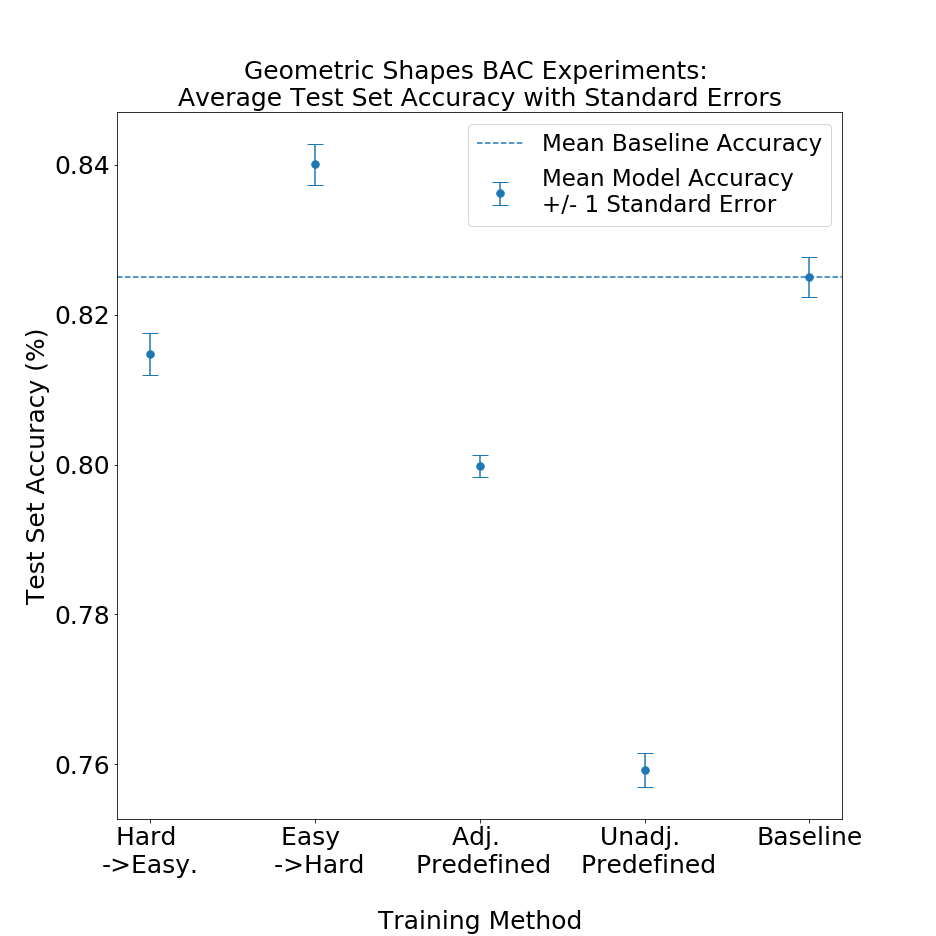
\includegraphics[width=1\linewidth]{GeoShapesBACResults_STE.png}
  \caption{ Mean Test Set Accuracies}
  \label{fig:BAC_StE}
\end{subfigure}%
\begin{subfigure}{0.7\textwidth}
\hspace*{-1cm}   
  \centering
  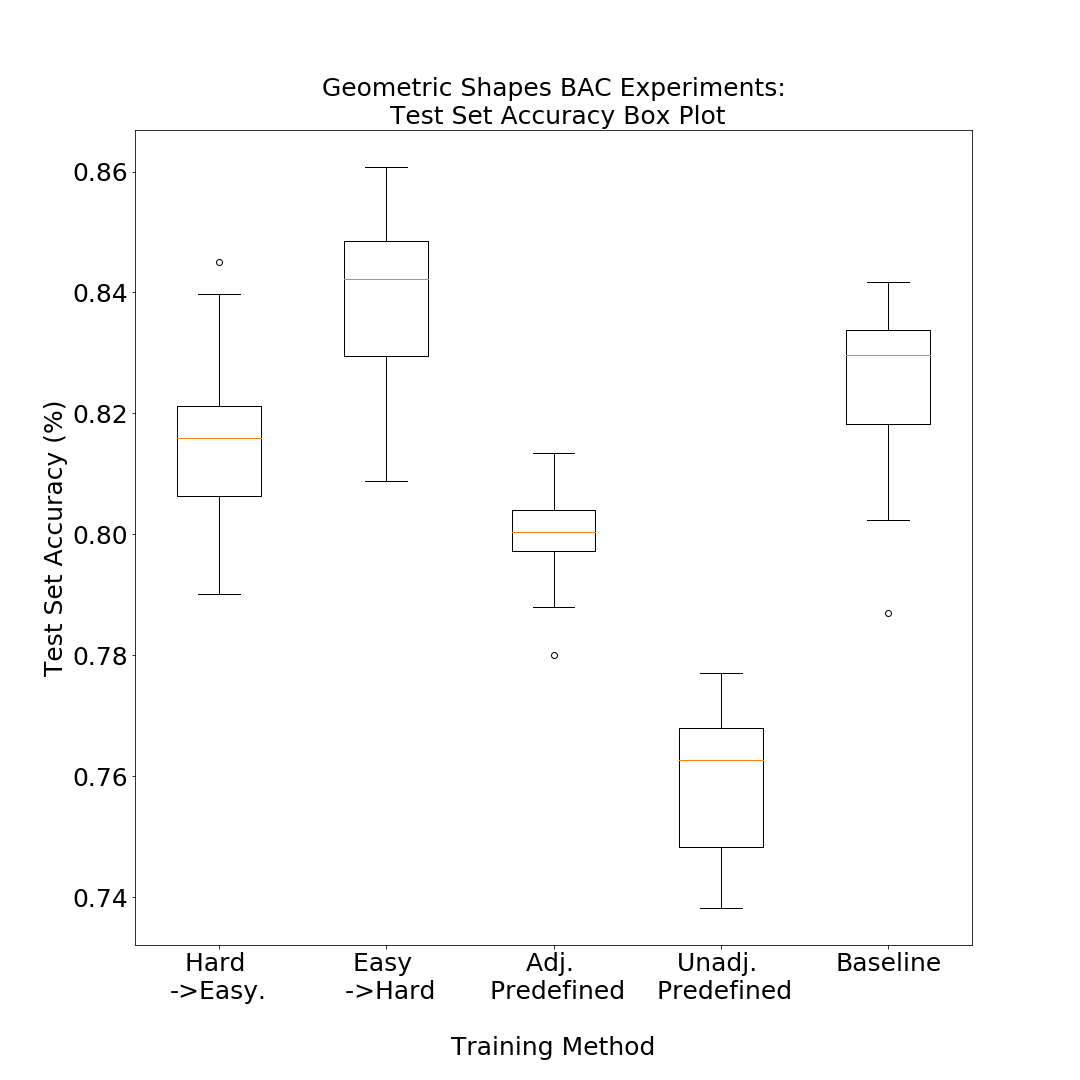
\includegraphics[width=1\linewidth]{GeoShapesBACResults_Boxplt.png}
  \caption{Test Set Accuracy Boxplots}
  \label{fig:BAC_Boxplt}
\end{subfigure}
\caption{Geometric Shapes Bootstrapped Active Curriculum (BAC) Experiment Results}
\label{fig:GeoShapesBACResults}
\end{figure}

We see from the results that the Easy to Hard curriculum model significantly outperforms the baseline model, with an average test accuracy improvement of around 2.5\%, over 5 standard errors, higher than the baseline test performance.  Cross-entropy error is also reduced, with the Easy to Hard curriculum test error over 6 standard errors below that of the baseline model. These results suggest that, not only is there a benefit to training the model with a curriculum, the BAC model seems to be succesful at identifying which samples should be used in the different curriculum learning phases. Conversely, the other curriculum methods all underperform the baseline model; the Hard to Easy curriculum in some ways acts as a control, showing that the improvement in the Easy to Hard model is driven by the order in which the tasks are included in training, as opposed to being a consequence of another part of the BAC method. It is interesting to note that both of the predefined curriculum models underperform the baseline model; the lower accuracy of the unadjusted method would seem to support the authors' suggestion in  \cite{Bengio2009} that the performance differences in their experiments may have been a result of their curriculum model having seen overall more training samples than their baseline. However, even our adjusted version of the predefined curriculum results in a significantly lower test accuracy than the baseline. This is interesting as this method is effectively trained in the same way as the BAC approach, however the tasks are predetermined by an intuitive sense of difficulty, as opposed to being derived from the baseline. This would suggest that, even for datasets where there as a somewhat clear distinction between hard and easy samples, a bootstrapped curriculum may be more useful. Potentially, this may because the BAC method specifically calculates which samples the model itself is uncertain in classifying, as opposed to assuming that our intuitive sense of difficulty corresponds to the best curriculum for the model. We would note however, that given the relatively low resolution of the images (as illustrated in Figure \ref{fig:GeoSamples}), there is perhaps less observable difference between the easy and hard training sets than might be assumed, and that this may contribute to the poor performance of the predefined curriculum.

With that in mind, we can analyse one of the the Easy to Hard curriculum experiments in more depth, in order to ascertain which samples are included in the two tasks. Recall that in the BAC method we train a baseline model, then use the uncertainty in the model's output class probabilities for the training samples, calculated using the AADT function defined in Section\ref{BAC_AADT}, to score and rank the training samples. The training samples are then split into two tasks, the first consisting of the training samples that the model is least uncertain in classifying, and the second task containing the samples about which the model's outputs are most uncertain. We can analyse the composition of the two tasks to infer which samples the model is least/most uncertain about. Doing so for one of the experiments presents some interesting conclusions; first of all, there is a significant lack of balance in the target classes in the two tasks. In task 1, the easier task, 43\% of the images are of triangles, while 31\% are of ellipses and 26\% are of rectangles, implying that the baseline model is significantly more confident in classifying whether or not an image shows a triangle than it is in classifying the other shapes. The bottom right image in Figure \ref{fig:HardGeoSamples} illustrates why this may be, with an example of an ellipse that looks quite similar to a mis-shapen rectangle, again this is probably the result of the low resolution of the images. We also observe that 64\% of the samples in the first task are from the easy training set of squares, circles and equilateral triangles, showing that the AADT function is somewhat succesful in separating the two training sets, however the first task still contains a substantial number of the harder samples. In appendix REF APPENDIX, we show a number of samples from either task, illustrating how the first, easier task is predominantly made up of regular shapes, as well as triangle, which appear to be easier to classify than rectangles and ellipses. 

A potential enhancement to the BAC method would be to control the balance of the classes in either task, however if one class is indeed easier than the others to classify then it may be better for it to be over-represented in the easier task(s). While we used two tasks for the Geometric Shapes dataset as this corresponded to the number of tasks of the predefined curriculum, we also ran some initial experiments with a larger number of tasks. We found some variation in results with a larger number of tasks, with some choices of task number underperforming the baseline model, however further tests could be carried out in future work to ascertain how robust these results are and investigate what is driving the different performances.
\section{Summary}
To summarize, these experiments seem to support the hypothesis that training a deep model with a curriculum can reduce generalization error, and furthermore that using an active learning approach to inferring sample difficulty through model prediction uncertainty can be an effective way of automatically constructing such curricula. In particular such curriculum construction methods may even outperform a preconstructed curriculum using an intuitve sense of sample difficulty, as model uncertainty incorporates information about which samples the model itself finds difficult. One of the arguable drawbacks to the BAC method is that it requires that a baseline model is trained to convergence, in order to use its outputs to construct the curriculum to train the curriculum model. This effectively doubles the training time and, while this may not be too significant a computational burden in some problems, motivates the approach of the next chapter, which investigates whether or not a curriculum can be constructed dynamically throughout training, without first training a baseline model.



